\documentclass[11pt,a4paper]{article}
\usepackage[margin=1.8cm,top=1.6cm,bottom=1.8cm]{geometry}
\usepackage[T1]{fontenc}
\usepackage{lmodern}
\usepackage{microtype}
\usepackage{amsmath}
\usepackage{graphicx}
\usepackage{booktabs}
\usepackage{caption}
\usepackage[hidelinks]{hyperref}
\captionsetup{font=small,labelfont=bf,skip=3pt}
\setlength{\parskip}{2pt}
\setlength{\parindent}{1em}
\setlength{\textfloatsep}{8pt plus 2pt minus 2pt}
\setlength{\floatsep}{6pt plus 2pt minus 2pt}
\newcommand{\code}[1]{\texttt{#1}}

\title{\vspace{-1.2cm}Seeing a Graph: one t-SNE gradient with Barnes--Hut,\\in parallel with Pthreads, OpenMP and OpenCilk}
% TODO: your name and AEM
\author{Your Name (AEM 0000) --- Parallel \& Distributed Computer Systems 2026, Homework 1\\
\small Code and data: \url{https://github.com/xristos05/pds-hw1}}
\date{\vspace{-0.9cm}}

\begin{document}
\maketitle

\section{Approach}

We compute $\partial C/\partial y_i = 4(F^{\mathrm{attr}}_i - F^{\mathrm{rep}}_i)$ at the given state $Y_0$, with $u=10$ and $\theta=0.5$.
The code is split in two parts. One file, \code{kernels.h}, holds the work for a single row, point, leaf or chunk; all versions share it.
Four small backends (\code{seq.c}, \code{omp.c}, \code{pth.c}, \code{cilk.c}) only decide which thread runs which chunk.
Every chunk size is fixed, and $Z$ is summed per chunk of 256 points and then over the chunks in order.
We compile with \code{-ffp-contract=off}, so gcc and clang round the same way.
As a result the four versions give \emph{bit-identical} $\beta$, $F^{\mathrm{attr}}$, $F^{\mathrm{rep}}$ and $Z$ for every number of threads; the benchmark script checks this for every version.

\textbf{Graph and $P$.} $W$ is symmetric, so its CSC form read from the file is also its CSR form. Column indices are stored as \code{int32} to halve the index traffic, and $P$ is stored with the same pattern as $W$.
For row $i$ we bisect on $\beta_i$ using $\ell_k=\log(w_{ik}/\max_k w_{ik})\le 0$, so $e^{\beta\ell_k}\le1$ and nothing overflows. The entropy is $H=\log S-\beta\sum_k e^{\beta\ell_k}\ell_k/S$ with $S=\sum_k e^{\beta\ell_k}$; we stop when $|H-\log\min(u,d_i)|<10^{-5}$.
Uniform rows skip the bisection. This covers every row of an unweighted graph.
Symmetrization finds the entry $(j,i)$ by binary search in the sorted row $j$. It is a separate parallel loop after a barrier, because row $i$ reads $p_{i|j}$ from row $j$.

\textbf{Attraction} is $F^{\mathrm{attr}}_i=\sum_j A_{ij}(y_i-y_j)$, with $A_{ij}=p_{ij}/(1+d_{ij}^2)$ computed on the fly. This is a sparse $\times$ dense ($n\times2$) product.
It streams \code{col} and \code{P} once and gathers $y_j$ at random, so it does $O(\mathrm{nnz})$ work at about 12 bytes per handful of flops.

\textbf{Quadtree: fixed depth.} The leaves form a $2^L\times2^L$ grid over the bounding square. Level $l$ is a dense array of $4^l$ cells, numbered in Morton (Z-order), so the children of cell $c$ are $4c,\dots,4c{+}3$.
Each cell stores its point count and its center of mass. A counting sort orders the points by leaf; because of the Morton order, the points of \emph{every} cell at every level are then contiguous in memory.
The parallel counting sort is stable and has five steps. (1)~Each thread finds the bounding box of one block of points. (2)~Each thread computes the leaf codes of its block and a histogram of leaves. (3)~We total each block of 4096 leaves and scan these totals. (4)~We compute the start of each leaf and the first slot of each thread inside each leaf. (5)~Each thread scatters its points.
Stability makes the order identical to the sequential sort. Centers of mass are computed from the leaves upward, one parallel loop per level; levels with fewer than 4096 cells run sequentially.

\textbf{Walk.} Each point uses an explicit stack. A cell is accepted when $r^2_{\text{diag}}<\theta^2 d^2$, compared as squares so no square root is needed. Inside a leaf, the points are added one by one and the point itself is skipped by its sorted index.
A cell that contains $y_i$ is never accepted, because there $d\le r_{\text{diag}}$, so $r/d\ge1>\theta$.
The points are walked in Morton order, in chunks of 256. Consecutive points open almost the same cells, which keeps them in cache.

\textbf{The three models.} \emph{OpenMP:} \code{schedule(dynamic,256)} for $P$, the attraction and the walk, because rows and points vary in cost: degrees run from 1 to 3{,}299, and points in dense regions open more cells. The tree build uses \code{static} blocks, one per thread, and the scans use \code{single}.
\emph{Pthreads:} threads are created at each parallel loop. They take chunks from a shared counter with \code{\_\_atomic\_fetch\_add}, which is dynamic scheduling, and the join acts as the barrier. One-block-per-thread loops use the same helper.
\emph{OpenCilk:} \code{cilk\_for} over the same chunks with \code{grainsize 1}, balanced by work stealing. The worker count is set through \code{CILK\_NWORKERS} (see the bug in Section~\ref{sec:bug}).

\textbf{Machine.} AMD Ryzen 7 5700X, 8 cores and 16 hardware threads (SMT), 4\,MB L2 and 32\,MB L3. Ubuntu 24.04 under WSL2 with 15\,GiB of RAM visible. gcc 13.3 (OpenMP, Pthreads) and OpenCilk 3.0 (clang 19.1.7), with \code{-O3 -march=native -ffp-contract=off}.
Each time is the fastest of 5 runs; file reading is not timed. Raw data: \code{results/*.csv}; plots: \code{scripts/plots.py}.

\section{Correctness}
Compared with the reference files, $\beta$ agrees to $1.2\cdot10^{-4}$ on \code{k49\_norm\_10NN}, which is the bisection tolerance; the unweighted graphs have uniform rows, so $\beta=0$ exactly. $F^{\mathrm{attr}}$ agrees to $1.3\cdot10^{-5}$ on k49 and to round-off ($2\cdot10^{-15}$) on the unweighted graphs.
At $\theta=0.5$ the error of $F^{\mathrm{rep}}$ ($\max|x-x_{\mathrm{ref}}|/\max|x_{\mathrm{ref}}|$) is $8.9\cdot10^{-3}$, $8.1\cdot10^{-3}$ and $5.6\cdot10^{-3}$ on k49, com-Amazon and coPapersDBLP; the relative error of $Z$ is $5.1$, $4.8$ and $3.6\cdot10^{-3}$.
At $\theta=0.1$ these errors fall below $6\cdot10^{-5}$ ($F^{\mathrm{rep}}$) and $3\cdot10^{-5}$ ($Z$), which shows that the remaining error is the approximation itself, not a defect in the code.
The direct $O(n^2)$ sum agrees with the reference to $1.2\cdot10^{-4}$, the accuracy of the reference itself, which was computed with Barnes--Hut at $\theta=0.1$.

\section{Results}

\begin{figure}[t]
\centering
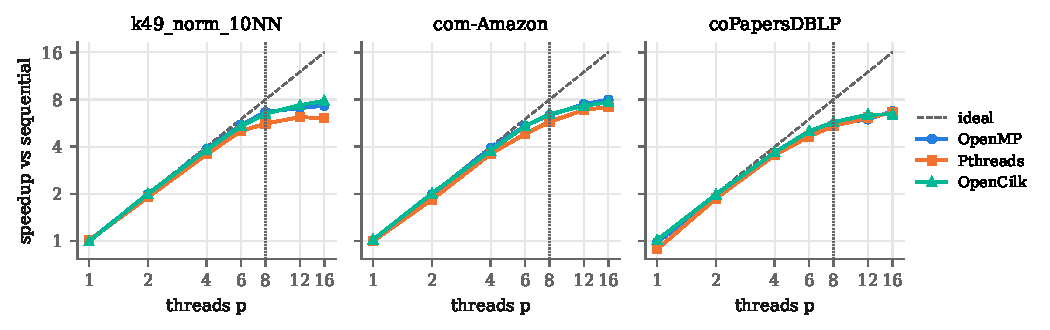
\includegraphics[width=\textwidth]{figs/speedup.pdf}
\caption{Speedup of the whole gradient (all phases) over the sequential version. The dotted line marks the 8 physical cores; beyond it, two threads share a core.}
\label{fig:speedup}
\end{figure}

\begin{figure}[t]
\centering
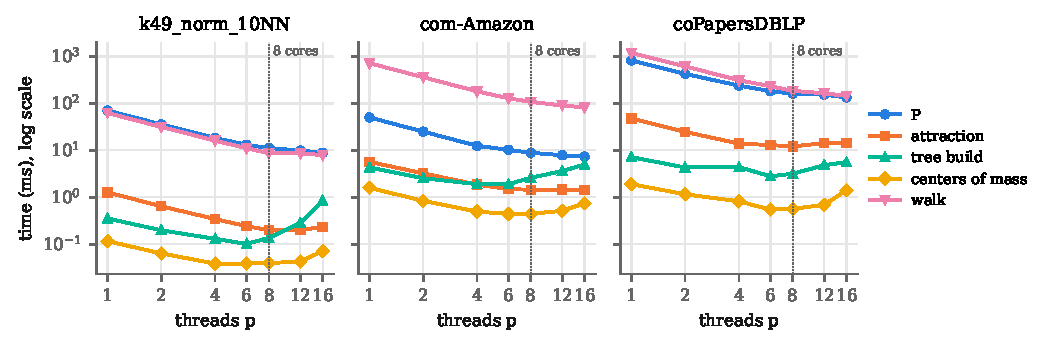
\includegraphics[width=\textwidth]{figs/phases.pdf}
\caption{Time of each phase against the number of threads (OpenMP; Pthreads and OpenCilk are similar, see \code{results/timings.csv}).}
\label{fig:phases}
\end{figure}

\begin{table}[t]
\centering\small
\begin{tabular}{l r r r r r r r r r}
\toprule
 & \multicolumn{3}{c}{k49\_norm\_10NN} & \multicolumn{3}{c}{com-Amazon} & \multicolumn{3}{c}{coPapersDBLP}\\
\cmidrule(lr){2-4}\cmidrule(lr){5-7}\cmidrule(lr){8-10}
phase & $p{=}1$ & $p{=}16$ & $S$ & $p{=}1$ & $p{=}16$ & $S$ & $p{=}1$ & $p{=}16$ & $S$\\
\midrule
P & 70.9 & 8.90 & 8.0 & 49.7 & 7.36 & 6.8 & 782.4 & 133.56 & 5.9\\
attraction & 1.3 & 0.23 & 5.4 & 5.5 & 1.44 & 3.8 & 46.0 & 14.13 & 3.3\\
tree build & 0.3 & 0.86 & 0.4 & 4.5 & 5.00 & 0.9 & 7.0 & 5.65 & 1.2\\
centers of mass & 0.1 & 0.07 & 1.6 & 1.6 & 0.75 & 2.1 & 1.9 & 1.41 & 1.4\\
walk & 62.5 & 7.94 & 7.9 & 715.3 & 81.97 & 8.7 & 1183.1 & 144.79 & 8.2\\
\midrule
total & 135.3 & 18.53 & 7.3 & 778.1 & 97.63 & 8.0 & 2021.5 & 300.56 & 6.7\\
\bottomrule
\end{tabular}

\caption{Phase times in ms, sequential ($p{=}1$) and OpenMP with 16 threads, and the speedup $S$. Graph sizes: $n=$ 38{,}547 / 334{,}863 / 540{,}486; $\mathrm{nnz}=$ 0.62\,M / 1.85\,M / 30.5\,M.}
\label{tab:phases}
\end{table}

All three models reach a speedup of 6.1--8.0 on the whole gradient at 16 threads (Fig.~\ref{fig:speedup}).
OpenMP and OpenCilk are within a few percent of each other. Pthreads is slower on the smallest graph because it creates threads at every parallel loop; on k49 each phase takes only a few milliseconds.
Up to 4 threads the speedup is close to ideal, and at 8 threads it is 5.4--6.7. Beyond 8, the hardware threads share cores, and the extra gain is small (Fig.~\ref{fig:phases}, Table~\ref{tab:phases}). The phases scale differently:

\textbf{Walk}, 7.9--8.7$\times$. This is the largest phase and it is compute-bound: each point does independent work on a tree that fits in cache. It scales almost linearly up to 8 cores, and SMT adds another 10--30\%: two threads on one core hide each other's memory latency while walking the tree. Its cost grows as $n\log n$: 1.62, 2.14 and 2.19\,$\mu$s per point.
\textbf{$P$.} On k49 the bisection is compute-bound and scales 8.0$\times$. On the unweighted graphs, $P$ is only the symmetrization: about 26\,ns per nonzero, mostly binary searches into random rows, which are cache misses. Its speedup drops to 6.5$\times$ (Amazon) and 5.9$\times$ (DBLP, whose 0.6\,GB of arrays do not fit in the 32\,MB L3).
\textbf{Attraction}, only 3.3--5.4$\times$. It is memory-bound: on DBLP, 30.5\,M nonzeros $\times$ 12 bytes stream in 14\,ms, about 26\,GB/s plus the gathers of $y_j$. More cores do not add memory bandwidth, so its speedup stops near $p=6$ (Fig.~\ref{fig:phases}).
The rows differ greatly in length (DBLP degree 1 to 3{,}299). Dynamic chunks of 256 rows balance them; with static rows, one thread would get many more nonzeros. Long rows also amortize the per-row overhead, so DBLP costs 1.5\,ns per nonzero against 3.0 on Amazon.
\textbf{Tree build and centers of mass} take a few milliseconds and barely scale (0.4--1.6$\times$). The per-thread histograms cost $O(p\cdot4^L)$, which grows with $p$; the upper levels of the tree are small and run sequentially, with a barrier per level. Pthreads pays for creating threads at each of the 5 loops of the build. Together these phases take at most 5\% of the time, so their poor scaling hardly affects the total.

\begin{figure}[t]
\centering
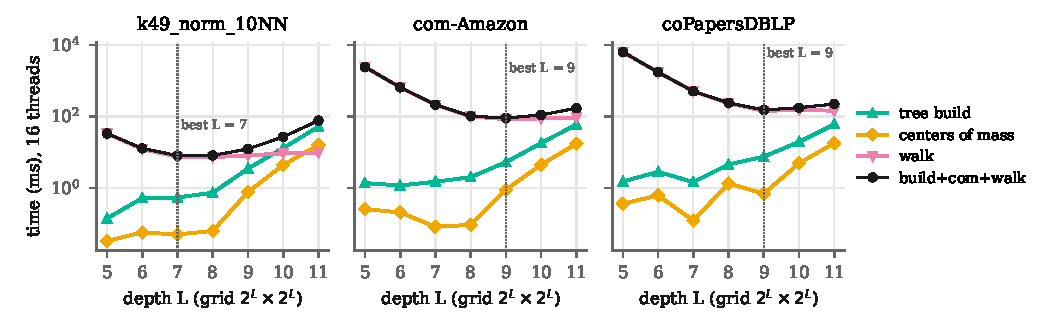
\includegraphics[width=\textwidth]{figs/depth.pdf}
\caption{Tree depth $L$ against time (OpenMP, 16 threads). Too shallow: long direct sums in crowded leaves. Too deep: many cells to visit, and the build grows as $p\cdot4^L$.}
\label{fig:depth}
\end{figure}

\textbf{Choice of depth $L$} (Fig.~\ref{fig:depth}). The best depth is $L=7$ ($128\times128$) for k49 and $L=9$ ($512\times512$) for com-Amazon and coPapersDBLP, which is 3--4 points per occupied leaf.
With fewer levels the walk is up to 45$\times$ slower: on DBLP at $L=5$ it takes 6.4\,s instead of 0.14\,s, because every leaf holds hundreds of points that are summed directly. With more levels the walk visits more cells, and the build at 16 threads grows from 7.5\,ms ($L=9$) to 61\,ms ($L=11$).
We therefore choose $L=\lceil\log_4(n/4)\rceil$ (about 4 points per leaf), which picks the best $L$ for all three graphs. It also adapts to graphs of a million nodes, giving $L=9$ or $10$.

\begin{figure}[t]
\centering
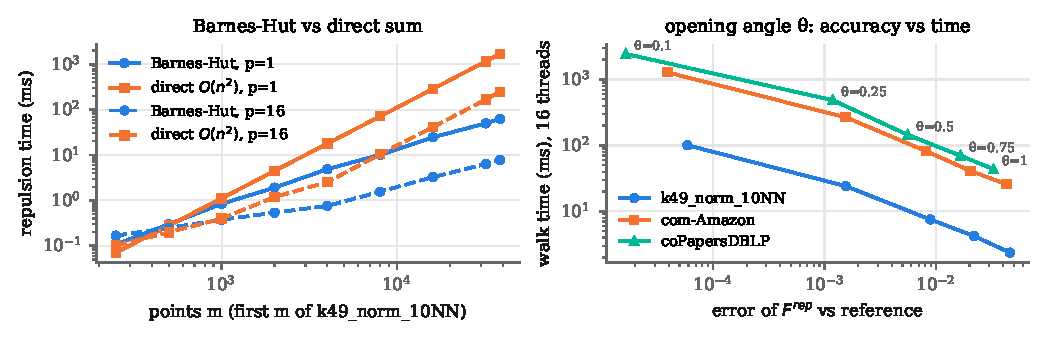
\includegraphics[width=\textwidth]{figs/crossover_theta.pdf}
\caption{Left: repulsion time on the first $m$ points of k49, Barnes--Hut (build + centers of mass + walk) against the direct sum. Right: opening angle $\theta\in\{0.1,0.25,0.5,0.75,1\}$, accuracy against walk time.}
\label{fig:cross}
\end{figure}

\textbf{Barnes--Hut against the direct sum} (Fig.~\ref{fig:cross}, left). On k49 the parallel direct $O(n^2)$ sum takes 1.68\,s on 1 thread and 0.247\,s on 16. Barnes--Hut takes 0.063\,s and 0.0083\,s, which is \textbf{27$\times$ and 30$\times$ faster}.
The direct sum grows as $m^2$ and Barnes--Hut as about $m\log m$; the two cross between $m=500$ and $1000$ points for both 1 and 16 threads. Below that, the direct sum wins: no tree to build, and a simple inner loop.
\textbf{$\theta$} (Fig.~\ref{fig:cross}, right) trades accuracy for time. From $\theta=0.1$ to $1$ the walk becomes 42--56$\times$ faster and the error grows from $10^{-5}$ to $4\cdot10^{-2}$. At $\theta=0.5$ the error is below $10^{-2}$ on all three graphs.

\section{Predict, then measure: coPapersDBLP}

\begin{table}[t]
\centering\small
\begin{tabular}{l l r r r r}
\toprule
phase & model & pred.\ $p{=}1$ & meas. & pred.\ $p{=}16$ & meas.\\
\midrule
P & $\propto$ nnz & 770 & 819 & 150 & 134\\
attraction & $\propto$ nnz & 90 & 48 & 15 & 14\\
tree build & $a n + b 4^L$ & 6 & 7 & 5.0 & 5.6\\
centers of mass & $\propto 4^L + n$ & 2 & 2 & 0.6 & 1.4\\
walk & $c\, n \log_2 n$ & 1160 & 1179 & 140 & 145\\
\midrule
total &  & 2000 & 2056 & 310 & 301\\
\bottomrule
\end{tabular}

\caption{coPapersDBLP, OpenMP, times in ms. The prediction was committed to the repository (\code{results/prediction-dblp.md}) before the run.}
\label{tab:pred}
\end{table}

We predicted each phase from the per-unit costs measured on k49 and com-Amazon (Table~\ref{tab:pred}).
DBLP has 1.6$\times$ more nodes than com-Amazon but 16.5$\times$ more nonzeros, and the same $L=9$.
The walk was predicted from $c\,n\log_2n$, with $c$ fitted on the two smaller graphs ($c=0.110$ and $0.115\,\mu$s). That came within 2\%, which confirms that the walk does not depend on the edges.
$P$ was predicted from the cost per nonzero on com-Amazon and came within 6\%; its speedup was lower than on Amazon, as we expected once the arrays no longer fit in L3.
The miss was the \emph{sequential} attraction, measured at half the prediction. Its cost per nonzero is not constant: com-Amazon has a median degree of 4, so its per-row overhead (loading $y_i$, storing $F_i$, starting a short loop) is spread over few nonzeros, while DBLP's median degree is 34.
At 16 threads, however, the prediction was right (14\,ms), because there the limit is memory bandwidth, which does not depend on row length. Overall the total came within 3\% (2.06\,s against 2.0\,s) at $p=1$ and 3\% (301\,ms against 310\,ms) at $p=16$.

\section{One bug}\label{sec:bug}
In the first full run, OpenCilk with $p=1$ took 0.019\,s on k49. That is the same as OpenMP with 16 threads and 7$\times$ faster than the sequential version, and it held at every $p$. One worker cannot be faster than the sequential code, so the number itself was the clue.
A 5-line test printed \code{\_\_cilkrts\_get\_nworkers()} after \code{setenv("CILK\_NWORKERS","1")} inside \code{main}: it reported all hardware threads.
The OpenCilk runtime starts \emph{before} \code{main} and reads the variable then, so our call to \code{setenv} was too late, and every ``Cilk, $p$ threads'' run had used 16 workers.
The fix: \code{backend\_init} sets the variable and restarts the program with \code{execv} if the variable was not already right, then aborts unless the runtime reports exactly $p$ workers.
After the fix, Cilk at $p=1$ matches the sequential version (0.137\,s against 0.135\,s), and the whole benchmark was re-run. Lesson: always check that $p=1$ matches the sequential time.

\section{Use of AI assistants}
% TODO: rewrite in your own words; be specific about what YOU checked and changed.
I used Claude (Anthropic) to write the first version of the code and of the benchmark and plotting scripts, and to draft this report from my measurements.
I ran every measurement on my machine and checked every number against the raw CSV files. The Cilk bug of Section~\ref{sec:bug} was in the AI-generated code; I caught it from the impossible 1-thread timing in my results.

\small
\noindent\textbf{References.}
[1] L.~van der Maaten, Accelerating t-SNE using tree-based algorithms, \emph{JMLR} 15, 2014.
[2] J.~Barnes, P.~Hut, A hierarchical $O(N\log N)$ force-calculation algorithm, \emph{Nature} 324, 1986.
\end{document}
